\documentclass[11pt]{article}

\usepackage[margin=2.5cm]{geometry}
\usepackage{amsmath,amssymb,mathtools}
\usepackage{booktabs,array}
\usepackage{xcolor}
\usepackage{tikz}
\usetikzlibrary{arrows.meta,positioning,calc}
\usepackage{pgfplots}
\pgfplotsset{compat=1.18}
\usepackage{algorithm}
\usepackage{algpseudocode}
\usepackage[colorlinks=true,linkcolor=blue!50!black,citecolor=blue!50!black,urlcolor=blue!50!black]{hyperref}

\newcommand{\R}{\mathbb{R}}
\newcommand{\norm}[1]{\left\lVert #1 \right\rVert}
\newcommand{\code}[1]{\texttt{#1}}
\newcommand{\xh}{\hat{x}}
\DeclareMathOperator{\sym}{sym}
\DeclareMathOperator{\diag}{diag}
\algrenewcommand\algorithmicrequire{\textbf{Input:}}
\algrenewcommand\algorithmicensure{\textbf{Output:}}

\title{HGDL: Methodology and Implementation}
\date{1 October 2026 --- describes \code{hgdl} 2.4 plus the changes listed as \emph{Unreleased} in \code{CHANGELOG.md}}

\begin{document}
\maketitle

\begin{abstract}
HGDL (Hybrid Global Deflated Local) searches a differentiable function for many optima at once
and returns a growing, sorted list of \emph{unique} optima rather than a single answer. It
combines distributed local optimizations (``walkers''), deflation of every optimum already
found so that it is not found again, and a global (genetic) step that places new walkers. This
document describes the mathematics of each component, how several deflations are combined,
how constraints are treated, and how the method is implemented and executed asynchronously on
a dask cluster. Pseudocode follows the code closely; Section~\ref{sec:map} maps every concept
to the function that implements it.
\end{abstract}

\tableofcontents

%======================================================================
\section{Problem and notation}
%======================================================================

HGDL considers
\begin{equation}\label{eq:problem}
  \min_{x \in \Omega} f(x) \quad\text{subject to}\quad c^L \le c(x) \le c^U,
  \qquad \Omega = \{x \in \R^D : l \le x \le u\},
\end{equation}
where $f:\R^D\to\R$ is twice differentiable with gradient $g = \nabla f$ and Hessian
$H = \nabla^2 f$, and the (optional) constraints $c:\R^D\to\R^m$ have Jacobian $J$; an equality
constraint has $c^L_i = c^U_i$, a one-sided constraint an infinite bound. The user supplies $f$
and $g$; $H$ is optional and otherwise replaced by forward differences of $g$
(step $10^{-6}$, upper triangle mirrored).

Instead of a single minimizer, HGDL returns a list
\[
  \mathcal{L} = \big\{(x_k,\ f(x_k),\ \text{class}_k,\ \lambda_k,\ g_k,\ r_k)\big\}_k ,
\]
sorted by $f(x_k)$, where $\lambda_k$ are curvature eigenvalues, $g_k$ the gradient (of the
Lagrangian under constraints) and $r_k$ the deflation radius. Two modes decide what is sought:
\begin{description}
  \item[minimization] (default) strict local minima, with any local optimizer;
  \item[stationary points] all non-degenerate stationary points (minima, maxima, saddle
  points), with the built-in Newton method and without constraints.
\end{description}
The list is never truncated, because it doubles as the set of deflation points: the subset
\[
  \mathcal{D} = \{(x_k, r_k) \in \mathcal{L} : \text{class}_k \in
  \{\text{minimum}, \text{maximum}, \text{saddle point}\}\}
\]
is deflated (Section~\ref{sec:deflation}). The user-facing limit \code{number\_of\_optima} only
limits how many entries \code{get\_latest()}/\code{get\_final()} return.

The box $\Omega$ is the domain from which starting points are drawn. It is \emph{not} treated as
a constraint in the sense of~\eqref{eq:problem}: bound-respecting scipy optimizers keep their
iterates in $\Omega$, the built-in Newton method only projects onto it, and users are advised
to choose wide bounds.

%======================================================================
\section{Overview}\label{sec:overview}
%======================================================================

A \emph{walker} is one local optimization started from a point $x^0$. HGDL keeps one walker
running on every worker thread of a dask cluster. Whenever a walker finishes:
\begin{enumerate}
  \item its result is judged: is it an acceptable optimum (Section~\ref{sec:accept}), and is it
  new, i.e.\ not inside the deflation radius of a known optimum?
  \item if so, it is classified, inserted into $\mathcal{L}$ and, from then on, deflated;
  \item a new walker is started, from a point proposed by the global step
  (Section~\ref{sec:global}), and it sees the deflation set as it is at that moment.
\end{enumerate}
The run ends after $N_{\text{epochs}} \times N_w$ walkers have finished, where $N_w$ is the
number of walkers at the start (the number of worker threads). There is no synchronization
between walkers (Section~\ref{sec:async}); the name \code{num\_epochs} is kept from the earlier,
epoch-synchronized design and now only sets the length of the run.

Every walker optimizes a \emph{deflated} problem: the gradient and Hessian it sees are
modified so that they blow up near every known optimum (Section~\ref{sec:deflation}). Which
results are accepted, however, is always decided on the \emph{true} derivatives.

%======================================================================
\section{Local search: the walker}\label{sec:local}
%======================================================================

A walker receives a start $x^0$, the problem, and a snapshot of the deflation set
$\{(\xh_k, r_k)\}_{k=1}^K$. It builds the deflated gradient $G$ and deflated Jacobian $J_G$
(Section~\ref{sec:deflation}) and calls one of three local optimizers:

\begin{description}
  \item[\code{dNewton}] HGDL's Newton iteration on $G(x) = 0$ (Algorithm~\ref{alg:dnewton}).
  In stationary-point mode it takes the plain Newton step $s = -J_G^{-1} G$ (least squares if
  $J_G$ is singular) and converges to any nearby stationary point. In minimization mode it takes
  the \emph{saddle-free} step~\cite{dauphin2014}
  \begin{equation}\label{eq:saddlefree}
    s = -\,V \diag\!\big(1/\max(|\theta_i|, \varphi)\big) V^T G,
    \qquad \sym(J_G) = \tfrac12 (J_G + J_G^T) = V \diag(\theta) V^T,
  \end{equation}
  with the floor $\varphi = 10^{-8}\max(1, \max_i|\theta_i|)$. Because $|\sym(J_G)|$ is positive
  definite, $s$ is a descent direction and the iteration is repelled by maxima and saddle points.
  Iterates are projected onto $\Omega$; the iteration stops when both the step and $G$ are
  below the tolerance, after \code{local\_max\_iter} (default 1000) iterations, or on a
  non-finite step.
  \item[scipy] any method of \code{scipy.optimize.minimize}, called with the \emph{true}
  objective $f$, the deflated gradient $G$ as \code{jac} and $J_G$ as \code{hess}, the bounds
  and constraints. With constraints, HGDL always uses SLSQP.
  \item[callable] a user function \code{f(func, grad, hess, bounds, x0, *args)} returning a
  scipy-like result; it receives the deflated derivatives as well.
\end{description}

The walker then judges its own result (Section~\ref{sec:accept}) and returns
$(x, f(x), g, \lambda, r, \text{success})$.

%======================================================================
\section{Deflation}\label{sec:deflation}
%======================================================================

\subsection{One bump}

Deflation follows the HGDN method of Noack and Funke~\cite{noack2017}. Around a known optimum
$\xh$ with radius $r$, the bump function (Eq.~(7) of~\cite{noack2017} with radial support,
$\alpha = r^2$) is
\begin{equation}\label{eq:bump}
  \beta(x; \xh, r) =
  \begin{cases}
    \exp\!\big(1 - 1/a(x)\big), & a(x) = 1 - \norm{x-\xh}^2/r^2 > 0,\\[2pt]
    0, & \text{otherwise.}
  \end{cases}
\end{equation}
It is $C^\infty$, equal to $1$ at $\xh$, strictly between $0$ and $1$ inside the ball
$\norm{x - \xh} < r$, and $0$ outside. Its gradient is
\begin{equation}\label{eq:bumpgrad}
  \nabla\beta(x) = -\,\frac{2\,\beta(x)}{a(x)^2\, r^2}\,(x - \xh).
\end{equation}

\subsection{Several deflations: the product operator}

With $K$ deflation points the \emph{deflation operator} is the product
\begin{equation}\label{eq:D}
  \mathcal{D}(x) = \prod_{k=1}^{K} \frac{1}{1 - \bar\beta_k(x)},
  \qquad \bar\beta_k = \min\big(\beta(x;\xh_k,r_k),\ \beta_{\max}\big),
  \quad \beta_{\max} = 1 - 10^{-5},
\end{equation}
and the deflated gradient and its Jacobian are
\begin{align}
  G(x) &= \mathcal{D}(x)\, g(x), \label{eq:G}\\
  J_G(x) &= \mathcal{D}(x)\, H(x) + g(x)\, \nabla\mathcal{D}(x)^T,
  \qquad
  \nabla\mathcal{D} = \mathcal{D} \sum_{k=1}^K \frac{\nabla\beta_k}{1 - \bar\beta_k}. \label{eq:JG}
\end{align}
(In Eq.~\eqref{eq:JG} the code uses $\nabla\beta_k$ of the uncapped bump; the cap only keeps
the denominator away from zero.) $J_G$ is the exact Jacobian of $G$ and is not symmetric.

Each factor of~\eqref{eq:D} is $\ge 1$, so $\mathcal{D} \ge 1$ everywhere and $\mathcal{D} = 1$
outside all balls: deflation only rescales the gradient, it never changes its direction.
Overlapping balls simply multiply. An additive operator $1/(1 - \sum_k \beta_k)$ would not be
safe: where two bumps overlap, $\sum_k \beta_k$ can exceed $1$, the operator changes sign, and a
deflated region turns into an attracting one. Figure~\ref{fig:deflation}(a) shows both.
Because all $K$ bumps are evaluated together (vectorized over the deflation points), one
evaluation of $\mathcal{D}$ costs $O(KD)$.

\begin{figure}[t]
\centering
\begin{tikzpicture}
\begin{axis}[width=0.48\textwidth, height=5.2cm, xlabel={$x$}, ymin=0, ymax=3.2,
  title={(a) two bumps, $\xh=0$, $r=1$ and $\xh=0.8$, $r=0.7$}, title style={font=\small},
  legend style={font=\scriptsize, at={(0.98,0.98)}, anchor=north east}, legend columns=3,
  tick label style={font=\scriptsize}]
  \addplot[blue, thick] table[x=x, y=b1] {figures/bumps.dat};
  \addplot[blue!60, thick, dashed] table[x=x, y=b2] {figures/bumps.dat};
  \addplot[red, thick, dotted] table[x=x, y=bsum] {figures/bumps.dat};
  \addplot[black, thick, domain=-1.5:2.5] {1};
  \legend{$\beta_1$, $\beta_2$, $\beta_1+\beta_2$ (exceeds 1)}
\end{axis}
\end{tikzpicture}\hfill
\begin{tikzpicture}
\begin{axis}[width=0.48\textwidth, height=5.2cm, xlabel={$x$}, ymin=-25, ymax=25,
  title={(b) $f'(x)$ and $\mathcal{D}f'$ for $f=(x^2-1)^2$, $\xh=1$, $r=0.5$}, title style={font=\small},
  legend style={font=\scriptsize, at={(0.02,0.98)}, anchor=north west}, tick label style={font=\scriptsize},
  unbounded coords=jump]
  \addplot[black, thick] table[x=x, y=fp] {figures/deflated_derivative.dat};
  \addplot[red, thick] table[x=x, y=Dfp] {figures/deflated_derivative.dat};
  \addplot[gray, thin, domain=-1.6:1.6] {0};
  \legend{$f'$, $\mathcal{D}\,f'$}
\end{axis}
\end{tikzpicture}
\caption{(a) Bumps~\eqref{eq:bump} of two overlapping deflation balls. Their sum exceeds 1
where they overlap, which would flip the sign of an additive operator; the product
operator~\eqref{eq:D} stays $\ge 1$. (b) The derivative of the double well and its deflated
version with the root $\xh = 1$ deflated: away from $\xh$ the two coincide (the roots $-1$ and $0$
are untouched), near $\xh$ the deflated derivative grows without bound instead of crossing zero.
The radius $0.5$ is enlarged for visibility (HGDL would use $1/f''(1) = 1/8$).}
\label{fig:deflation}
\end{figure}

\subsection{Behaviour near a deflated point}\label{sec:nearxh}

Let $e = x - \xh$, $d = \norm{e} \ll r$, and assume one bump is active and $g(\xh) = 0$. From
$1/a = 1 + d^2/r^2 + O(d^4/r^4)$ we get $\beta = \exp(-d^2/r^2 + O(d^4/r^4))$ and therefore
\begin{equation}\label{eq:asymp}
  1 - \beta \approx \frac{d^2}{r^2}, \qquad
  \mathcal{D} \approx \frac{r^2}{d^2}, \qquad
  \nabla \ln \mathcal{D} \approx -\frac{2e}{d^2}, \qquad
  g \approx H e .
\end{equation}
Consequently $\norm{G} \approx (r^2/d^2)\norm{He} \ge r^2 |\lambda|_{\min} / d \to \infty$: the
root of $g$ at $\xh$ is removed (Figure~\ref{fig:deflation}(b)).

\paragraph{The Newton step moves away from $\xh$.}
The Newton equation $J_G s = -G$ is, after dividing by $\mathcal{D}$,
$\big(H + g\, \nabla\ln\mathcal{D}^T\big) s = -g$. Inserting~\eqref{eq:asymp},
\[
  H\Big(I - \frac{2\,e e^T}{d^2}\Big)\, s = -H e .
\]
The matrix $R = I - 2ee^T/d^2$ is a Householder reflection ($R^2 = I$, $Re = -e$), so
$s = -R\,e = e$: the Newton step goes from $x = \xh + e$ to $\xh + 2e$, straight away from the
deflated point, doubling its distance. This is the mechanism by which deflated Newton walkers
leave the neighbourhood of known solutions; we verified it numerically with HGDL's
implementation of~\eqref{eq:G}--\eqref{eq:JG} ($s/e = 0.9999$ at $d = 10^{-2}r$).

\paragraph{The cap.}
With $\beta_{\max} = 1 - 10^{-5}$, $\mathcal{D} \le 10^5$ per bump; by~\eqref{eq:asymp} the cap
is reached for $d \lesssim r\sqrt{10^{-5}} \approx 3\cdot 10^{-3} r$. The cap keeps $\mathcal{D}$
finite, but it also means that $G(\xh) = \mathcal{D}(\xh)\,g(\xh) = 0$: $\xh$ remains a root of
$G$ inside a tiny ball. A walker that lands there is rejected by the arrival test of
Section~\ref{sec:arrival}.

\subsection{How deflation acts on the different local optimizers}\label{sec:defl-methods}

Deflation changes only the derivatives, never $f$, and $G$ is a positive multiple of $g$.
Whether a walker started in the basin of a deflated minimum leaves that basin therefore depends
on the local optimizer:
\begin{itemize}
  \item \textbf{Plain Newton} (stationary-point mode) steps away from $\xh$, as shown above.
  \item \textbf{Saddle-free Newton} (minimization mode): $|\sym(J_G)|$ is positive definite, so
  the step~\eqref{eq:saddlefree} satisfies $g^T s < 0$ and is a descent direction \emph{for $f$
  itself}. Near $\xh$, $J_G \approx \mathcal{D} H R$ with the reflection $R$ above, so
  $e^T \sym(J_G)\, e \approx -\mathcal{D}\, e^T H e < 0$: deflation creates negative curvature
  along $e$. Taking absolute values of the eigenvalues turns the step from $+e$ into
  approximately $-e$ (numerically $s^Te/\norm{e}^2 = -0.99$): the walker is pulled back to $\xh$.
  \item \textbf{Line-search quasi-Newton methods} (L-BFGS-B, SLSQP, \ldots) evaluate the true
  $f$ but the rescaled gradient $G$. The inconsistent pair distorts their step lengths and
  curvature updates; walkers leave the deflated ball but often stall without converging.
\end{itemize}
Table~\ref{tab:defl-methods} quantifies this on the four-well function
$f = (x_1^2-1)^2 + (x_2^2-1)^2$ with only the minimum $(1,1)$ deflated and 100 walkers started
in its basin. In minimization mode, uniqueness of the reported minima therefore rests on the
arrival test, not on deflation; Section~\ref{sec:limits} discusses a remedy for the saddle-free
step.

\begin{table}[t]
\centering
\caption{Where 100 walkers started uniformly in $(0.05, 1.95)^2$, the basin of the deflated
minimum $(1,1)$ of the four-well function, end up (radius $r = 1/8$).}
\label{tab:defl-methods}
\begin{tabular}{llrrr}
\toprule
mode & optimizer & back at $(1,1)$ & elsewhere stationary & not converged \\
\midrule
stationary points & plain Newton & 1 & 99 & 0 \\
minimization & L-BFGS-B & 0 & 34 & 66 \\
minimization & saddle-free Newton & 100 & 0 & 0 \\
\bottomrule
\end{tabular}
\end{table}

\subsection{The deflation radius}\label{sec:radius}

An accepted point $x$ with curvature eigenvalues $\lambda$ (Section~\ref{sec:accept}) gets
\begin{equation}\label{eq:radius}
  r = \min\!\Big(\frac{1}{\lambda_*},\ \rho\,\norm{u - l}\Big), \qquad
  \lambda_* = \begin{cases} \min_i \lambda_i & \text{minimization},\\ \min_i |\lambda_i| & \text{stationary points},\end{cases}
  \qquad \rho = 0.1 .
\end{equation}
At a stationary point the principal curvatures of the graph of $f$ are exactly the Hessian
eigenvalues, so $1/\lambda_*$ is the largest principal radius of curvature (the osculating
circle in the flattest direction) --- an estimate of the extent of the optimum. Like every
curvature of the graph it depends on the scale of $f$; this is deliberate. The cap keeps a
single poorly conditioned optimum from deflating the whole domain.

%======================================================================
\section{Accepting and classifying results}\label{sec:accept}
%======================================================================

\subsection{Unconstrained problems}

A walker's result $x$ with returned (deflated) gradient $\hat g$ is a \emph{local success} if
\begin{equation}\label{eq:accept}
  \hat g \text{ finite}, \qquad \norm{\hat g} < \varepsilon_g = 10^{-6}, \qquad
  \lambda_* > \varepsilon_\lambda = 10^{-6},
\end{equation}
where $\lambda$ are the eigenvalues of the true, symmetrized Hessian $\sym(H(x))$ and
$\lambda_*$ is defined in~\eqref{eq:radius}. Since $\mathcal{D} \ge 1$, the condition on
$\hat g$ implies $\norm{g} < 10^{-6}$. Points that fail are returned with $r = 0$ and are not
inserted into $\mathcal{L}$ (with one exception, Section~\ref{sec:first}).

\subsection{Classification}

An inserted point is classified from its gradient $g$ and eigenvalues $\lambda$, in this order:
\begin{center}
\begin{tabular}{ll}
\toprule
condition & class \\
\midrule
$\max_i |g_i| > 10^{-3}$ & degenerate \\
$\min_i |\lambda_i| < 10^{-5}$ & zero curvature \\
all $\lambda_i > 0$ & minimum \\
all $\lambda_i < 0$ & maximum \\
mixed signs & saddle point \\
\bottomrule
\end{tabular}
\end{center}
Only minima, maxima and saddle points are deflated.

\subsection{The arrival test}\label{sec:arrival}

A successful result $x$ with gradient $g$ is rejected as a duplicate if it lies inside the ball
of a known deflation point:
\begin{equation}\label{eq:arrival}
  \exists\, k:\ \norm{x - \xh_k} < r_k \ \text{ and }\ \max_i |g_i| < 10^{-5}.
\end{equation}
The test is applied in the coordinator against the deflation set \emph{at the time the result
arrives}, which may be larger than the set the walker started with (Section~\ref{sec:async}).

%======================================================================
\section{Constraints}\label{sec:constraints}
%======================================================================

With constraints the walker always runs SLSQP. Its result generally lies on active
constraints, where $g \ne 0$; the tests~\eqref{eq:accept} would reject it. Constrained results
are therefore judged by the Karush--Kuhn--Tucker (KKT) conditions~\cite{nocedal2006}.

\subsection{Constraint representation}

All forms accepted by \code{scipy.optimize.minimize} (\code{NonlinearConstraint},
\code{LinearConstraint}, dictionaries of type \code{eq}/\code{ineq}) are normalized into blocks
$c^L \le c(x) \le c^U$; dictionary constraints become $c(x) \ge 0$ or $c(x) = 0$. Derivatives
the user does not supply are approximated:
\begin{itemize}
  \item $J$ by central differences, step $h_i = 10^{-6}\max(1, |x_i|)$;
  \item the weighted Hessian $\sum_i w_i \nabla^2 c_i$ from the user's \code{hess(x, w)} if
  given; else by central differences of $J^T w$ (symmetrized) if $J$ is given; else by second
  differences of $w^T c$ with step $10^{-4}\max(1,|x_i|)$ --- differencing a difference quotient
  would lose half the significant digits.
\end{itemize}
The box $\Omega$ is not part of the constraints.

\subsection{First-order conditions: multipliers by bounded least squares}

At $x$, with tolerances $\tau_i = 10^{-6}\max(1, |\text{bound}_i|)$:
\begin{align*}
  \mathcal{E} &= \{i : c^L_i = c^U_i\} && \text{(equalities)},\\
  \mathcal{A}^L &= \{i \notin \mathcal{E} : c^L_i \text{ finite},\ c_i(x) - c^L_i \le \tau_i\}
     && \text{(active lower bounds)},\\
  \mathcal{A}^U &= \{i \notin \mathcal{E} : c^U_i \text{ finite},\ c^U_i - c_i(x) \le \tau_i\}
     && \text{(active upper bounds)},
\end{align*}
$\mathcal{A} = \mathcal{E} \cup \mathcal{A}^L \cup \mathcal{A}^U$, and $x$ is \emph{feasible}
if every constraint is satisfied within $\tau_i$. At a local minimum of~\eqref{eq:problem},
$g = J_{\mathcal{A}}^T w$ with $w_i \ge 0$ on $\mathcal{A}^L$ (moving into the feasible side
would increase $f$), $w_i \le 0$ on $\mathcal{A}^U$, and $w_i$ free on $\mathcal{E}$. HGDL
computes the multipliers from the true gradient,
\begin{equation}\label{eq:bvls}
  w_{\mathcal{A}} = \arg\min_{w}\ \norm{J_{\mathcal{A}}^T w - g}
  \quad\text{s.t.}\quad w_i \ge 0\ (i\in\mathcal{A}^L),\ \ w_i \le 0\ (i\in\mathcal{A}^U),
\end{equation}
($w_i = 0$ for inactive constraints) with bounded-variable least squares~\cite{stark1995}, the
same way for every local optimizer, and forms the gradient of the Lagrangian
$L = f - w^T c$:
\begin{equation}\label{eq:gradL}
  \nabla L(x) = g(x) - J(x)^T w .
\end{equation}
The sign bounds in~\eqref{eq:bvls} matter: a point where $g$ points out of the feasible set
(so that $f$ decreases into it) cannot be balanced with admissible multipliers and keeps a
large $\nabla L$. Without active constraints, $\nabla L = g$.

\subsection{Second-order conditions and the radius}

Let $\mathcal{S} = \mathcal{E} \cup \{i \in \mathcal{A} : |w_i| > 10^{-8}\}$ be the strongly
active constraints and $Z$ an orthonormal basis of the null space of $J_{\mathcal{S}}$ (the
tangent space). The curvature that decides about a minimum is that of the Lagrangian along the
tangent space,
\begin{equation}\label{eq:reduced}
  \mu = \operatorname{eig}\!\Big( Z^T \big(\sym(H) - \textstyle\sum_i w_i \nabla^2 c_i\big) Z \Big),
\end{equation}
a vector of length $D - \operatorname{rank} J_{\mathcal{S}}$. The result is accepted if it is
feasible, $\norm{\nabla L} < 10^{-6}$, and $\min \mu > 10^{-6}$; if the strongly active
constraints fix $x$ completely ($Z$ empty, e.g.\ a vertex with positive multipliers), the
first-order conditions suffice. The radius is~\eqref{eq:radius} with $\lambda = \mu$, and the
cap $\rho\norm{u-l}$ when $Z$ is empty. The reported \code{df/dx} is $\nabla L$ and the reported
eigenvalues are $\mu$, so the classification table above applies unchanged. Weakly active
constraints ($w_i \approx 0$) are left out of $\mathcal{S}$, which makes the second-order test
conservative.

\subsection{Newton polish on the KKT system}\label{sec:polish}

SLSQP stops when $f$ stops changing; near an optimum this leaves $\norm{\nabla L}$ around the
square root of its tolerance ($\approx 10^{-5}$), above $\varepsilon_g$. Before the test,
HGDL therefore applies up to five Newton steps to the KKT system of the strongly active
constraints with targets $t_i$ (the bound each one sits on),
\begin{equation}\label{eq:kktnewton}
  \begin{bmatrix} \nabla^2 L & -J_{\mathcal{S}}^T \\ J_{\mathcal{S}} & 0 \end{bmatrix}
  \begin{bmatrix} \Delta x \\ \Delta w \end{bmatrix}
  = -\begin{bmatrix} \nabla L \\ c_{\mathcal{S}}(x) - t_{\mathcal{S}} \end{bmatrix},
\end{equation}
solved in the least-squares sense. Only $\Delta x$ is used: at the new point the active set and
the multipliers are recomputed with~\eqref{eq:bvls}. A step is kept only if the point stays
feasible and the residual norm of the right-hand side decreases; the polish is attempted only
at feasible points with $\norm{\nabla L} < 10^{-3}$, so it refines nearly converged walkers and
leaves stalled ones alone. Converging at the quadratic rate of Newton's method, one or two
steps take $\norm{\nabla L}$ from $10^{-5}$ to machine precision.

\subsection{Constraints and deflation}

Deflation is applied unchanged: SLSQP receives $G = \mathcal{D}\, g$. Mathematically a KKT point
of the original problem remains a KKT point of the deflated one ($\mathcal{D} g = J^T
(\mathcal{D} w)$); in practice SLSQP's line search on the undeflated $f$ stalls inside the
deflation ball, and these stalled walkers fail the KKT test. Walkers that do reach a known
optimum are rejected by the arrival test~\eqref{eq:arrival}, whose gradient condition uses
$\nabla L$. Constraints cannot be combined with stationary-point mode, since SLSQP is a
minimizer.

%======================================================================
\section{Global step}\label{sec:global}
%======================================================================

New walkers start from batches of $N_w$ points. Let $n = \min(|\mathcal{L}|, N_w)$ and let
$X \in \R^{n\times D}$, $y \in \R^n$ be the positions and values of the $n$ best entries of
$\mathcal{L}$. The global method proposes $n$ points, and the batch is padded with
$N_w - n$ points drawn uniformly from $\Omega$; the very first batch is the user's $x^0$, padded
or truncated in the same way.

\paragraph{Genetic step} (default; Algorithm~\ref{alg:genetic}). Values are mapped to
fitnesses that favour low $f$, $q_j = 2 - (y_j - \min y)/(\max y - \min y)$ (all $q_j = 1$ if
$y$ is constant), normalized to $p_j = q_j / \sum q$, and sharpened with the ``unfairness''
$\nu = 100$: $p_j \leftarrow p_j^{\nu-1} / \sum_i p_i^{\nu-1}$. Each child draws two parents
$m, d$ from $p$ (with replacement) and is their fitness-weighted average plus a small Gaussian
perturbation,
\[
  x_{\text{child}} = \frac{p_m X_m + p_d X_d}{p_m + p_d} + \xi, \qquad
  \xi \sim \mathcal{N}\big(0,\ \diag(\omega\,(u - l))^2\big), \quad \omega = 5\cdot 10^{-4}.
\]
Children outside $\Omega$ are replaced by uniform samples. Children therefore start near (or
between) the best known optima; deflation is what makes a walker started there move to a
\emph{different} optimum.

\paragraph{Random step.} The $n$ points are drawn uniformly from $\Omega$.

\paragraph{Callable.} A user function \code{(X, y, bounds, n)} returning $n$ points.

%======================================================================
\section{Asynchronous execution}\label{sec:async}
%======================================================================

\subsection{Coordinator and walkers}

\code{optimize()} is non-blocking. It sends one \code{Problem} object (objective, derivatives,
bounds, constraints, settings, run id) to every worker once, starts a coordinator thread in the
calling process, and returns. Walkers are ordinary dask tasks that receive a reference to that
object, their start point and a copy of the deflation set; dask places them on free worker
threads and re-runs them if a worker dies. All state --- the list $\mathcal{L}$ and the set of
pending tasks --- lives in the calling process and is changed only by the coordinator thread,
under a lock that \code{get\_latest()} also takes before returning a deep copy.

The coordinator (Algorithm~\ref{alg:coordinator}) keeps $N_w$ walkers in flight and consumes
them in completion order. There is no barrier: a slow or diverging walker occupies only its
own worker thread while all others continue (Figure~\ref{fig:timeline}). The number of walkers
is re-read every $N_w$ completions, so adaptive clusters may grow or shrink. The run ends when
$N_{\text{epochs}} N_w$ walkers have completed; walkers still running are then cancelled or
stopped, so \code{get\_final()} never waits for a straggler.

\begin{figure}[t]
\centering
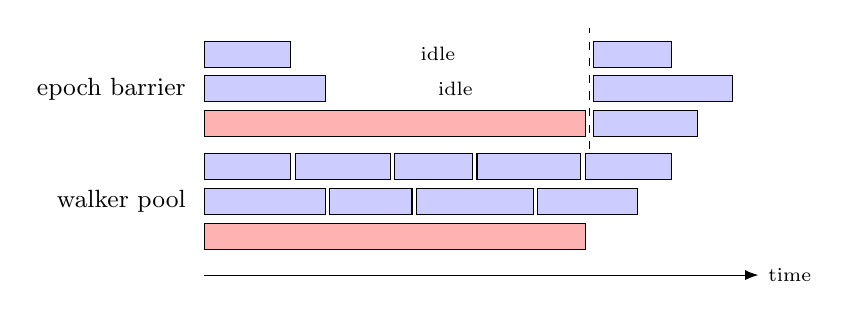
\begin{tikzpicture}[x=0.55cm, y=0.55cm, font=\scriptsize]
  \tikzset{w/.style={draw, fill=blue!20, minimum height=0.4cm}, s/.style={draw, fill=red!30}}
  \node[anchor=east] at (0,4.1) {\small epoch barrier};
  % barrier version: three threads, epoch length set by the slowest walker
  \draw[w] (0.2,4.6) rectangle (2.2,5.2); \draw[w] (9.2,4.6) rectangle (11.0,5.2);
  \draw[w] (0.2,3.8) rectangle (3.0,4.4); \draw[w] (9.2,3.8) rectangle (12.4,4.4);
  \draw[s] (0.2,3.0) rectangle (9.0,3.6); \draw[w] (9.2,3.0) rectangle (11.6,3.6);
  \draw[dashed] (9.1,2.7) -- (9.1,5.5);
  \node at (5.6,4.9) {idle}; \node at (6.0,4.1) {idle};
  \node[anchor=east] at (0,1.5) {\small walker pool};
  \draw[w] (0.2,2.0) rectangle (2.2,2.6); \draw[w] (2.3,2.0) rectangle (4.5,2.6);
  \draw[w] (4.6,2.0) rectangle (6.4,2.6); \draw[w] (6.5,2.0) rectangle (8.9,2.6);
  \draw[w] (9.0,2.0) rectangle (11.0,2.6);
  \draw[w] (0.2,1.2) rectangle (3.0,1.8); \draw[w] (3.1,1.2) rectangle (5.0,1.8);
  \draw[w] (5.1,1.2) rectangle (7.8,1.8); \draw[w] (7.9,1.2) rectangle (10.2,1.8);
  \draw[s] (0.2,0.4) rectangle (9.0,1.0);
  \draw[-{Latex}] (0.2,-0.2) -- (13,-0.2) node[right] {time};
\end{tikzpicture}
\caption{Three worker threads, one slow walker (red). With an epoch barrier (top) the other
threads wait for it; in the walker pool (bottom) they keep starting new walkers.}
\label{fig:timeline}
\end{figure}

\subsection{Consistency between walkers and the changing deflation set}

A walker never sees the live list. It receives a copy of the deflation points and radii when it
is submitted and optimizes one fixed deflated function from start to end, so no walker observes
the function change under it, and walkers share no mutable state. The price is staleness: a
walker does not know optima found after it started and may converge to one of them. Uniqueness
is therefore enforced where results arrive: the coordinator handles one completed walker at a
time and applies the arrival test~\eqref{eq:arrival} against the \emph{current} deflation set,
so if two walkers find the same new optimum, the first to arrive is inserted and the second is
rejected. (With an epoch barrier, all walkers of an epoch shared the snapshot taken at its
start; a walker's snapshot is now at least as recent.)

\subsection{The first results}\label{sec:first}

If none of the first $N_w$ completed walkers produced a successful result and $\mathcal{L}$ is
still empty, their results are inserted anyway (they are classified, typically as degenerate,
and not deflated). This guarantees that \code{get\_final()[0]} exists, which downstream users
rely on, e.g.\ when every optimum lies on the boundary of $\Omega$.

\subsection{Stopping and time limits}

Between two iterations, every walker asks a local watch whether to give up:
\begin{itemize}
  \item its \code{local\_time\_limit} (seconds, optional) has passed, or
  \item its run was stopped. \code{cancel\_tasks()} and the end of the run cancel the pending
  tasks and send one message to every worker (\code{client.run}) that records the run id in a
  set in the worker's memory; walkers check that set. This costs one message per worker, never
  a request per walker, and therefore scales to thousands of walkers.
\end{itemize}
scipy optimizers are stopped from their callback (SLSQP and TNC let the resulting
\code{StopIteration} escape; the walker then uses the last iterate), \code{dNewton} through a
hook in its loop. A stopped walker's result is judged like any other and usually rejected. A
single evaluation of $f$, $g$ or $H$ cannot be interrupted, and neither can a user-supplied
local optimizer.

\subsection{Reproducibility}

All random numbers are drawn in the coordinator. With one worker the run is reproducible for a
fixed seed; with several workers the completion order varies, so the set of optima found is
stable but the run is not bit-for-bit reproducible.

%======================================================================
\section{Pseudocode}\label{sec:pseudocode}
%======================================================================

\begin{algorithm}[H]
\caption{Coordinator (\code{HGDL.optimize}, \code{\_run\_walkers})}\label{alg:coordinator}
\begin{algorithmic}[1]
\Require $f, g, H$, bounds $[l,u]$, constraints, start points $x^0$, $N_{\text{epochs}}$
\State $N_w \gets$ number of worker threads; $Q \gets x^0$ padded/truncated to $N_w$ rows
\State send $\mathcal{P} = (f, g, H, l, u, \text{constraints}, \text{settings}, \text{run id})$ to all workers
\State $\mathcal{L} \gets \emptyset$; $n_c \gets 0$; $F \gets \emptyset$ \Comment{$F$: failed results among the first $N_w$}
\State \textbf{start} $N_w$ walkers \Comment{each via \textsc{Submit}}
\For{each walker result $\mathcal{R}$, in order of completion}
  \State \textbf{if} stopped \textbf{then break}
  \State $n_c \gets n_c + 1$
  \If{$\mathcal{R}$ successful \textbf{and} not rejected by the arrival test against current $\mathcal{D}$}
    \State classify $\mathcal{R}$, insert into $\mathcal{L}$ (sorted by $f$)
  \ElsIf{$n_c \le N_w$} \State $F \gets F \cup \{\mathcal{R}\}$
  \EndIf
  \If{$n_c = N_w$ \textbf{and} $\mathcal{L} = \emptyset$} \State insert all of $F$ into $\mathcal{L}$ \Comment{Section~\ref{sec:first}}
  \EndIf
  \State \textbf{if} $n_c \ge N_{\text{epochs}} N_w$ \textbf{then break}
  \State \textbf{if} $n_c \bmod N_w = 0$ \textbf{then} re-read $N_w$
  \State start walkers until $N_w$ are in flight
\EndFor
\State cancel pending walkers; mark the run stopped on every worker
\Statex
\Procedure{Submit}{}
  \If{$Q = \emptyset$} \State $Q \gets$ \Call{GlobalStep}{best $\min(|\mathcal{L}|,N_w)$ entries of $\mathcal{L}$} padded with uniform samples to $N_w$
  \EndIf
  \State pop $x_s$ from $Q$; start \Call{Walker}{$x_s, \mathcal{P}$, copy of $\mathcal{D}$} as a dask task
\EndProcedure
\end{algorithmic}
\end{algorithm}

\begin{algorithm}[H]
\caption{Walker (\code{local\_method})}\label{alg:walker}
\begin{algorithmic}[1]
\Require start $x_s$, problem $\mathcal{P}$, deflation set $\{(\xh_k, r_k)\}$
\State $G \gets \mathcal{D}\, g$, $J_G \gets \mathcal{D} H + g\nabla\mathcal{D}^T$ \Comment{Eqs.~\eqref{eq:D}--\eqref{eq:JG}}
\If{optimizer is \code{dNewton}} \State $x \gets$ \Call{DeflatedNewton}{$x_s$, saddle-free $=$ (mode is minimization)}
\Else \State $x \gets$ scipy \code{minimize}$(f, x_s, \texttt{jac}=G, \texttt{hess}=J_G$, bounds, constraints, callback$=$watch$)$ or user callable
\EndIf
\If{constraints}
  \State $x \gets$ \Call{NewtonPolish}{$x$} \Comment{Algorithm~\ref{alg:kkt}}
  \State $(\hat g, \lambda, \text{feasible}) \gets$ \Call{KKT}{$x$} \Comment{$\hat g = \nabla L$, $\lambda = \mu$}
\Else
  \State $\hat g \gets$ gradient returned by the optimizer; $\lambda \gets \operatorname{eig}(\sym H(x))$; feasible $\gets$ true
\EndIf
\State $\lambda_* \gets \min\lambda$ (minimization) or $\min|\lambda|$ (stationary points); $\lambda_* \gets \infty$ if $\lambda$ is empty
\State success $\gets$ feasible $\wedge$ $\hat g$ finite $\wedge$ $\norm{\hat g} < 10^{-6}$ $\wedge$ $\lambda_* > 10^{-6}$
\State $r \gets \min(1/\lambda_*, 0.1\norm{u-l})$ if success, else $0$
\State \Return $(x, f(x), \hat g, \lambda, r, \text{success})$
\end{algorithmic}
\end{algorithm}

\begin{algorithm}[H]
\caption{Deflated Newton (\code{DNewton})}\label{alg:dnewton}
\begin{algorithmic}[1]
\Require $x$, $G$, $J_G$, bounds, tolerance $t$, iteration limit $N$, saddle-free flag, watch
\State $s \gets \infty$, $k \gets 0$
\While{$\norm{s}_\infty > t$ \textbf{or} $\norm{G(x)}_\infty > t$}
  \State $x \gets \Pi_{[l,u]}(x)$ \Comment{projection onto the box}
  \If{saddle-free} \State $s \gets$ step~\eqref{eq:saddlefree}
  \Else \State $s \gets -J_G(x)^{-1} G(x)$ \Comment{least squares if singular}
  \EndIf
  \State \textbf{if} $s$ not finite \textbf{then return} $x$, failure
  \State $x \gets x + s$; $k \gets k + 1$
  \State \textbf{if} $k > N$ \textbf{or} watch says stop \textbf{then return} $x$, failure
\EndWhile
\State \Return $x$, converged
\end{algorithmic}
\end{algorithm}

\begin{algorithm}[H]
\caption{KKT test and Newton polish (\code{kkt\_conditions}, \code{newton\_polish})}\label{alg:kkt}
\begin{algorithmic}[1]
\Function{State}{$x$}
  \State evaluate $c(x)$, $J(x)$; determine $\mathcal{E}, \mathcal{A}^L, \mathcal{A}^U$ and feasibility
  \State $w \gets$ bounded least squares~\eqref{eq:bvls} on the true $g(x)$
  \State $\mathcal{S} \gets \mathcal{E} \cup \{i \in \mathcal{A} : |w_i| > 10^{-8}\}$
  \State \Return $c, J, w, \mathcal{S}$, feasible
\EndFunction
\Function{KKT}{$x$}
  \State $(c, J, w, \mathcal{S}, \text{feasible}) \gets$ \Call{State}{$x$}; $\nabla L \gets g - J^T w$
  \If{$\operatorname{null}(J_{\mathcal{S}}) = \{0\}$} \State \Return $\nabla L$, $\emptyset$, feasible
  \EndIf
  \State $Z \gets$ orthonormal basis of $\operatorname{null}(J_{\mathcal{S}})$
  \State \Return $\nabla L$, $\operatorname{eig}\big(Z^T(\sym H - \sum_i w_i \nabla^2 c_i) Z\big)$, feasible
\EndFunction
\Function{NewtonPolish}{$x$}
  \State $(c, J, w, \mathcal{S}, \text{feasible}) \gets$ \Call{State}{$x$}
  \State \textbf{if not} feasible \textbf{or} $\norm{g - J^Tw} \ge 10^{-3}$ \textbf{then return} $x$
  \For{at most 5 steps, while residual $> 10^{-12}$}
    \State solve~\eqref{eq:kktnewton} for $\Delta x$ (least squares); $x' \gets x + \Delta x$
    \State \textbf{if} $x'$ infeasible \textbf{or} its residual is not smaller \textbf{then break}
    \State $x \gets x'$; recompute \Call{State}{$x$}
  \EndFor
  \State \Return $x$
\EndFunction
\end{algorithmic}
\end{algorithm}

\begin{algorithm}[H]
\caption{Genetic step (\code{genetic\_step})}\label{alg:genetic}
\begin{algorithmic}[1]
\Require parents $X \in \R^{n\times D}$, values $y$, bounds, number of children $n$
\State $q_j \gets 2 - (y_j - \min y)/(\max y - \min y)$ \Comment{all $1$ if $y$ is constant}
\State $p \gets q/\sum q$; \ $p \gets p^{99} / \sum p^{99}$ \Comment{unfairness $\nu = 100$}
\For{each child}
  \State draw parents $m, d \sim p$
  \State $x \gets (p_m X_m + p_d X_d)/(p_m + p_d) + \mathcal{N}(0, \diag(5\cdot10^{-4}(u-l))^2)$
  \State \textbf{if} $x \notin \Omega$ \textbf{then} $x \gets$ uniform sample from $\Omega$
\EndFor
\end{algorithmic}
\end{algorithm}

%======================================================================
\section{Implementation map}\label{sec:map}
%======================================================================

\begin{center}
\small
\begin{tabular}{>{\raggedright\arraybackslash}p{0.36\textwidth}>{\raggedright\arraybackslash}p{0.57\textwidth}}
\toprule
concept & code \\
\midrule
user API, coordinator, walker pool, stopping & \code{hgdl/hgdl.py}: \code{HGDL}, \code{optimize}, \code{\_run\_walkers}, \code{\_submit\_walker}, \code{\_accept}, \code{\_stop\_walkers} \\
problem snapshot sent to the workers & \code{hgdl/problem.py}: \code{Problem}; default Hessian \code{approximate\_hessian} \\
walker, acceptance, radius, watch & \code{hgdl/local\_methods/local\_optimizer.py}: \code{local\_method}, \code{\_Watch}, \code{stop\_run} \\
arrival test & \code{local\_optimizer.py}: \code{collect\_results} \\
bump, deflation operator, $G$, $J_G$ & \code{hgdl/local\_methods/bump\_function.py}: \code{b}, \code{\_bumps}, \code{deflation\_and\_gradient}, \code{deflated\_grad}, \code{deflated\_hess} \\
deflated Newton, saddle-free step & \code{hgdl/local\_methods/dNewton.py}: \code{DNewton}, \code{saddle\_free\_step} \\
constraints: normalization, KKT, polish & \code{hgdl/local\_methods/kkt.py}: \code{normalize\_constraints}, \code{kkt\_conditions}, \code{newton\_polish} \\
list, classification, deflation set & \code{hgdl/optima.py}: \code{optima.fill\_in\_optima\_list}, \code{get\_deflation\_points} \\
global step & \code{hgdl/global\_methods/global\_optimizer.py}: \code{run\_global}, \code{genetic\_step}, \code{random\_step} \\
\bottomrule
\end{tabular}
\end{center}

\section{Constants}

\begin{center}
\small
\begin{tabular}{lll}
\toprule
quantity & value & where \\
\midrule
gradient threshold for success $\varepsilon_g$ & $10^{-6}$ & \code{local\_method} \\
curvature threshold $\varepsilon_\lambda$ & $10^{-6}$ & \code{local\_method} \\
radius cap $\rho$ (fraction of the domain diagonal) & $0.1$ & \code{MAX\_RADIUS\_FRACTION} \\
bump cap $\beta_{\max}$ & $1 - 10^{-5}$ & \code{BUMP\_CAP} \\
classifier: degenerate if $\max|g_i| >$ & $10^{-3}$ & \code{fill\_in\_optima\_list} \\
classifier: zero curvature if $\min|\lambda_i| <$ & $10^{-5}$ & \code{fill\_in\_optima\_list} \\
arrival test: gradient below & $10^{-5}$ & \code{collect\_results} \\
\code{dNewton} iteration limit (default) & 1000 & \code{DNEWTON\_DEFAULT\_MAX\_ITER} \\
\code{dNewton}/scipy tolerance (default) & $10^{-10}$ & \code{optimize(tolerance=)} \\
saddle-free eigenvalue floor & $10^{-8}\max(1,\max|\theta|)$ & \code{saddle\_free\_step} \\
constraint activity/feasibility tolerance & $10^{-6}\max(1,|\text{bound}|)$ & \code{ACTIVE\_TOL} \\
strongly active multiplier & $|w_i| > 10^{-8}$ & \code{MULTIPLIER\_TOL} \\
constraint finite-difference steps & $10^{-6}$, $10^{-4}$ (relative) & \code{FD\_STEP}, \code{FD2\_STEP} \\
Newton polish: attempted below / steps & $\norm{\nabla L} < 10^{-3}$ / 5 & \code{newton\_polish} \\
default Hessian forward-difference step & $10^{-6}$ & \code{approximate\_hessian} \\
genetic unfairness $\nu$ / perturbation $\omega$ & 100 / $5\cdot 10^{-4}$ & \code{genetic\_step} \\
\bottomrule
\end{tabular}
\end{center}

%======================================================================
\section{Differences from HGDN and open issues}\label{sec:limits}
%======================================================================

\paragraph{Deliberate differences from~\cite{noack2017}.}
The bump has radial support ($\alpha = r^2$) instead of a per-coordinate one; the deflation
operator is a product rather than a sum; the genetic step averages two parents with fitness
weights plus a small perturbation instead of gene crossover and mutation; and the inner loop of
the paper's Algorithm~4 (reset the walkers and repeat the deflated search until nothing new is
found) is not implemented --- each walker performs one local search and is replaced.

\paragraph{Deflation and the saddle-free step.}
As shown in Section~\ref{sec:defl-methods}, the saddle-free Newton step used in minimization
mode is a descent direction for $f$ and is not repelled by deflation. A preliminary experiment
(not implemented in \code{hgdl}) replaces it near deflated points by
\[
  s = -\big(|H| + g\,\nabla\ln\mathcal{D}^T\big)^{-1} g ,
\]
taking the absolute value of the eigenvalues of the true Hessian only. Far from all deflation
points ($\nabla\ln\mathcal{D} = 0$) this is the saddle-free step; near a deflated minimum
($|H| = H$) it is the plain Newton step of Section~\ref{sec:nearxh}, which moves away. In the
experiment of Table~\ref{tab:defl-methods} only 2 of 100 walkers returned to the deflated
minimum and 24 reached other minima, but most did not converge within 200 iterations; the
step needs further work before it can be adopted.

\paragraph{Bounds.} Optima on the boundary of $\Omega$ are not accepted, since $\Omega$ is not
treated as a constraint (Section~\ref{sec:first} keeps such runs from returning nothing).

\paragraph{Communication.} Every walker carries its copy of the deflation set; with
$10^4$ optima in high dimension this is megabytes per task. Scattering the set once and
passing references is a possible later optimization.

\begin{thebibliography}{9}
\bibitem{noack2017}
M.~M.~Noack and S.~W.~Funke.
\newblock Hybrid genetic deflated Newton method for global optimisation.
\newblock \emph{Journal of Computational and Applied Mathematics}, 325, 2017.

\bibitem{dauphin2014}
Y.~N.~Dauphin, R.~Pascanu, C.~Gulcehre, K.~Cho, S.~Ganguli and Y.~Bengio.
\newblock Identifying and attacking the saddle point problem in high-dimensional non-convex
optimization.
\newblock In \emph{Advances in Neural Information Processing Systems 27}, 2014.

\bibitem{nocedal2006}
J.~Nocedal and S.~J.~Wright.
\newblock \emph{Numerical Optimization}, 2nd ed.
\newblock Springer, 2006.

\bibitem{stark1995}
P.~B.~Stark and R.~L.~Parker.
\newblock Bounded-variable least-squares: an algorithm and applications.
\newblock \emph{Computational Statistics}, 10:129--141, 1995.
\end{thebibliography}

\end{document}
